\documentclass[a4paper,12pt]{article}
\usepackage{verbatim}
\usepackage[brazil]{babel}
\usepackage[utf8]{inputenc}
\usepackage{nomencl}
\usepackage{indentfirst}
\usepackage{hyperref}
\usepackage{textcomp}
\usepackage{graphicx}
\usepackage{wrapfig}


%\newcommand{\identacao}{\\[1mm] \hspace*{\parindent}}
\newcommand{\identacao}{\\[1mm] \hspace*{3cm}}
\hyphenation{pri-mei-ros}


\begin{document}

\title{Controle e Manutenção de Hortas e Jardins de Baixo Custo com Arduino}
\author{Gianluigi Dal Toso, Guilmour Rossi, Leandro Vieira, Luís Felipe\\Werlang, Mateus Gomes e Samuel Henrique\\\texttt{}\\\\\\
\multicolumn{1}{p{.95\textwidth}}{\centering\emph{Engenharia de Computação - Universidade Tecnológica Federal do Paraná (UTFPR) \\Oficina de Integração I}}}

\date{Curitiba, \\Junho de 2016}

\maketitle

\newpage


\tableofcontents


\newpage

\listoffigures

%\newpage

%\listoftables

\makenomenclature

\newpage
\section{Introdução}

O modelo atual de agricultura adotado nas últimas décadas, apesar de sua elevada efetividade de produção, tem se mostrado destrutivo ao planeta, com inúmeros impactos ambientais e também sociais; erosões do solo, contaminação de rios, redução da biodiversidade, exclusão social e etc. \cite[p.~23]{medeiros}. A fim de minimizar ou até eliminar estes problemas, novas alternativas de agricultura vem sendo buscadas e aperfeiçoadas, e com o avanço tecnológico e a consequente baixa de preços em componentes  eletrônicos, vê-se promissor a difusão de um sistema de controle e manutenção para jardins e hortas agroecológicas de baixo custo em quintais e apartamentos. Usando a plataforma de prototipagem eletrônica, \textit{Arduino}. Com o uso de sensores de umidade, temperatura, luz, e o correto manuseio dessas informações, pode-se encontrar as condições ideais para cultivo nestes locais, maximizando o crescimento e qualidade das plantas e garantindo um cultivo saudável mesmo em lares onde a manutenção de uma pequena horta não se encaixaria na rotina dos moradores.

Neste ponto  de um sistema de controle e manutenção para jardins e hortas agroecológicas e de baixo custo em quintais e apartamentos, usando a plataforma de prototipagem eletrônica, \textit{Arduino}. Com o uso de sensores de umidade, temperatura, luz, e o correto manuseio dessas informações, pode-se encontrar as condições ideais para cultivo nestes locais, maximizando o crescimento e qualidade das plantas e garantindo um cultivo saudável mesmo em lares onde a manutenção de uma pequena horta não se encaixaria na rotina dos moradores.

\textbf{\\Palavras-chave:} horta automatizada, jardim automatizado, arduino, monitoramento, hortas, automação residencial.


\newpage
\section{Metodologia}
\subsection{Fundamentos}

Uma primeira análise das necessidades do projeto nos indica que a solução a ser desenvolvida se assemelha mais à um sistema de controle do que à um software comercial. Não existem muitas entidades a serem tratadas pela aplicação, nem relações complexas entre elas. Também não há necessidade de se conectar em bases de dados nem se preocupar com erros do usuário. O programa é executado somente pela máquina e uma vez que ele esteja funcionando não há mais interação alguma com o usuário. Esses motivos nos fazem acreditar que a melhor estratégia para o desenvolvimento do projeto seja o uso da programação estruturada. Usar orientação a objetos é desnecessário para esse projeto e acabaria indo contra o próprio objetivo desse paradigma que é a simplificação do problema. TODO P(água) = P(bomba) - p.g.h
\subsection{Tecnologias}

O desenvolvimento de todo o código foi feito através da plataforma \textit{Arduino IDE} (Ambiente de Desenvolvimento Integrado, da sigla em Inglês), fornecida pelos próprios desenvolvedores do \textit{Arduino}. Essa IDE é simples e direta, e tenta suprir todas as necessidades para projetos de pequeno e médio porte; é possível verificar a integridade do código e enviar o mesmo para o \textit{Arduino}. Além disso, toda a sintaxe modificada da linguagem C++ para o Arduino é identificada pela IDE e ela ainda apresenta o \textit{Serial Monitor}, ferramenta com a qual é possível (após definição pelo código) receber informações da placa de prototipagem diretamente por um console na tela do computador. Para a organização do código utilizamos o controlador de versão e gerenciador de código-fonte \textit{git}, juntamente com a plataforma online \textit{Github}. Não houve uma máquina única utilizada para o desenvolvimento do projeto. Todas as ferramentas utilizadas são livres e funcionam em diferentes plataformas. Diferentes usuários, com diferentes hardwares e sistemas operacionais desenvolveram simultaneamente sem dificuldades. Praticamente qualquer computador moderno (fabricado pelo menos nos últimos dez anos) já é o suficiente para poder executar e colaborar no desenvolvimento do projeto.



\section{Recursos De Hardware E Software}
\subsection{Recursos de Hardware}

O principal recurso de hardware utilizado no projeto foi o controlador \textit{Arduino}, fornecido aos alunos pelo professor da disciplina juntamente com uma placa de ensaio (protoboard), cabos \textit{jumpers}, \textit{display} LED de sete segmentos (de quatro dígitos), mangueiras e terminais hidráulicos. Ademais, de contribuições dos membros da equipe, utilizamos uma fonte de 12V, cabos de tomada, uma lâmpada incandescente para o aquecimento,  e organizadores plásticos que serviram como estrutura para o projeto. Por fim, as aquisições extras necessárias consistiram de um módulo de relé de duas entradas para \textit{Arduino}, um sensor de temperatura DS18B20 à prova d’água, uma bomba hidráulica utilizada nos limpadores de para-brisa automotivos e também um sensor de umidade LM393 com sua sonda. Vale lembrar ainda que um dos membros forneceu também um módulo de \textit{ethernet} para o \textit{Arduino}, que apesar de suas funcionalidades não terem sido implementadas, está pronto para uso.\cite{igoe2007making}

\begin{figure}[!ht]
	\centering
		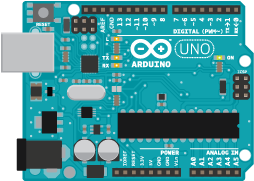
\includegraphics[width=0.5\textwidth]{illu-arduino-UNO.png}
		\caption{Placa Arduino Uno - para prototipagem eletrônica.}
\end{figure}


\subsection{Recursos de Software}

Graças ao fato de o \textit{Arduino} ser um hardware livre, o desenvolvimento para essa plataforma é bastante invetivado e difundido dentre estudantes, criadores e etc. Toda a programação do projeto foi feita na linguagem própria do \textit{Arduino} (C++ com pequenas modificações) utilizando a IDE fornecida pelos próprios desenvolvedores do hardware, a \textit{Arduino IDE}. Além disso, para organizar melhor, aumentar a eficiência do desenvolvimento e facilitar o trabalho em equipe, decidiu-se utilizar o sistema de controle de versão \textit{git} e hospedar o projeto no serviço \textit{Github}. Tanto a Arduino IDE, quanto a plataforma git são softwares de código-aberto e são oferecidas gratuitamente, funcionando na maioria dos sistemas operacionais modernos (\textit{Mac OS}, \textit{Windows} e \textit{Linux}).
    Apesar da linguagem C++ ser voltada ao desenvolvimento de projetos que envolvem a orientação a objetos, pode-se dizer que o nosso projeto foi desenvolvido de forma estruturada. A orientação à objetos foi utilizada apenas para a inicialização e calibragem do sensor de temperatura, e não foi utilizada como estratégia de resolução de problemas.

\begin{figure}[!ht]
	\centering
		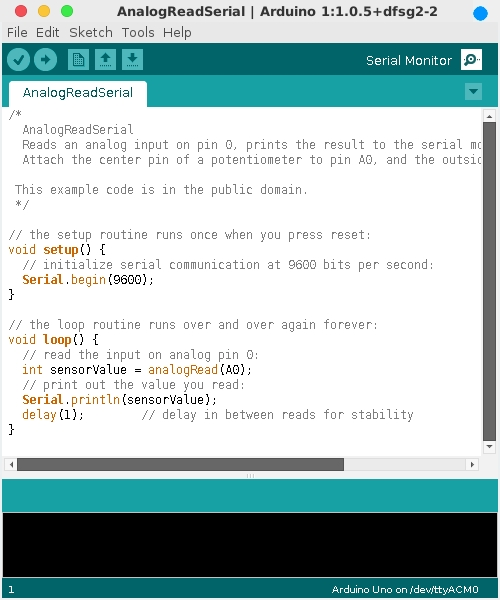
\includegraphics[width=0.8\textwidth]{arduinoIDE.jpg}
		\caption{Captura de Tela da Arduino IDE executada em Linux.}
\end{figure}

\subsection{Viabilidade}

A viabilidade do projeto é alta, pois este não envolve componentes de custo excessivo, nem exige uma capacidade técnica elevada. Por certo, com cerca de duzentos reais, se é capaz de adquirir todo os equipamentos e componentes necessários para a montagem de uma horta ou jardim automatizado. Quanto ao conhecimento técnico, este pode ser facilmente obtido através de inúmeros guias voltados à iniciantes disponíveis na \textit{internet} ou ainda nos milhares de livros e revistas guia para \textit{Arduino} facilmente encontrados em bancas ou até mesmo lojas de eletrônica. As informações contidas no presente relatório assim como os arquivos anexos à este projeto também tem o objetivo de facilitar a instalação e execução do projeto.



\section{Contexto}
\subsection{Publicação do Projeto}

O projeto inteiro será publicado \textit{online} pela equipe com o objetivo principal de aprendizado e também contribuir para a já vasta biblioteca de projetos desenvolvidos e criados na plataforma de prototipagem \textit{Arduino}. Todo o projeto será disponibilizado em código-aberto para que outras pessoas interessadas no assunto possam contribuir e/ou tirar suas dúvidas com o que já foi desenvolvido pela equipe.

\subsection{Licença}

Este e outros códigos criados por esta equipe para a disciplina CSX20 de Oficina de Integração I, da UTFPR, estão publicados sobre a \textit{MIT License}, que permite que qualquer um reaproveite o código da maneira que quiser, apenas garantindo o crédito intelectual pelo trabalho e não responsabilizando ou exigindo garantia de qualquer tipo pelo código original ou o gerado à partir deste. Os códigos-fonte do projeto estão disponíveis na internet pelo endereço: \href{http://github.com/guilmour/greew}{http://github.com/guilmour/greew}.




\section{Projeto a ser Desenvolvido e Resultados Iniciais do Mesmo}

\subsection{Projeto de Software}

O software criado  para o projeto foi desenvolvido utilizando programação estruturada, e como é comum em projetos de \textit{Arduino}, o código pôde ser dividido em três etapas. A primeira etapa consiste em definir as constantes que serão utilizadas durante a execução do programa. Aqui define-se as portas do \textit{Arduino} que serão utilizadas e também algumas configurações do programa. É nessa etapa por exemplo em que será definida a temperatura de ativação do aquecimento. Na segunda etapa, é executada a função \texttt{setup()} do \textit{Arduino}. Essa função é executada apenas uma vez e ela serve para definir quais portas representam entradas e quais representam saídas de dados (para proteção do circuito), além de inicializar o sensor de temperatura para que este possa funcionar corretamente. Por fim, a etapa final é a execução da função \texttt{loop().} Esta é executada em uma laço de repetição indeterminado e é onde as funcionalidades do projeto estão implementas.

    Esse laço de repetição nada mas é que uma função pré-exigida em todo programa para \textit{Arduino}, e é a parte principal do programa, sendo preciso ser executada em intervalos de tempo de curtíssima duração para que o \textit{display} LED funcione corretamente, uma vez que este não fica ligado constantemente, ele acende e apaga muito rapidamente de forma que o olho humano não seja capaz de perceber essa variação e perceba todos os dígitos acesos de forma contínua. Portanto, como era necessário que o \textit{loop} fosse executado com uma frequência alta, mas não era desejável que os sensores fossem monitorados em tal frequência, implementamos um programa que funciona em ciclos. Cada ciclo representa um número certo de iterações do \textit{loop} principal e portanto representa um certo intervalo de tempo. Dessa forma, podemos monitorar os sensores somente depois de executados um número propício de ciclos, sem que o \textit{display} seja afetado.

    Definido um número de ciclos a ser utilizado como base (ou intervalo base de tempo), o programa se encarrega de checar a leitura dos sensores de temperatura e de umidade do solo. A temperatura é então exibida no \textit{display} LED (a informação é repassada ao usuário) e o programa entra para a tomada de decisões: Se a temperatura ambiente estiver menor do que a definida na primeira etapa de execução do programa o relé referente à lampada incandescente será ativado e a mesma irá começar a esquentar o jardim, caso contrário este relé se mantêm desativado; Se a umidade do solo estiver abaixo do que o valor referente à um solo seco para aquela vegetação, o relé referente à bomba d’água será ativado e o jardim será irrigado até que o valor da umidade do solo esteja em um nível satisfatório.


\subsection{Projeto de Hardware}

    O componente central do hardware do projeto é a placa do \textit{Arduino Uno}. Esta fornece às calhas da \textit{protoboard} uma diferença de potencial de 5V que é utilizada pelos dois sensores do programa. O \textit{shield} \textit{ethernet} é acoplado ao \textit{Arduino}, com um de seus lados ocupando todas as portas digitais e analógicas da placa e do outro ele refornece às mesmas entradas. A \textit{protoboard} facilita a conexão dos componentes no \textit{Arduino}, que se organizam ficando o \textit{display} LED ocupando as dez primeiras portas digitais, o relé ocupando duas portas analógicas, o sensor de umidade também ocupando uma porta analógica e o sensor de temperatura ocupando uma porta digital. Um esquema da montagem final de todo o hardware do projeto pode ser conferida na imagem abaixo.

    No módulo do relé, uma das entradas será responsável por ligar a lâmpada incandescente e a outra por ligar a bomba d’água. Ambas as entradas podem ser ligadas de duas maneiras distintas, sendo elas “Comum - Normal Aberto” e “Comum - Normal Fechado”. Nos dois casos (lâmpada e bomba) optamos por fazer a ligação em Normal Aberto. Na ligação da lâmpada, uma das entradas da lâmpada foi ligada diretamente na rede e a outra é ligada na rede porém interrompida pelo relé. Já no caso da bomba d’água, os terminais da bomba são ligados com seus polos correspondentes na fonte de 12V, sendo um dos fios interrompidos pelo relé. É necessário por fim fornecer alimentação da rede para que a fonte funcione corretamente. Vale lembrar ainda que a fonte de 12V utilizada, se possuir mais de uma saída pode ainda ser utilizada também para fornecer energia ao \textit{Arduino}.

    Além disso existe o “\textit{hardware} físico” que foi desenvolvido para executar o projeto, que consistiu em adaptar a bomba d’água em um recipiente (e fazer a devida vedação), planejar e montar um circuito hidráulico e adaptar um contêiner físico para servir como modelo de jardim.


		\begin{figure}[!ht]
		  \centering
		    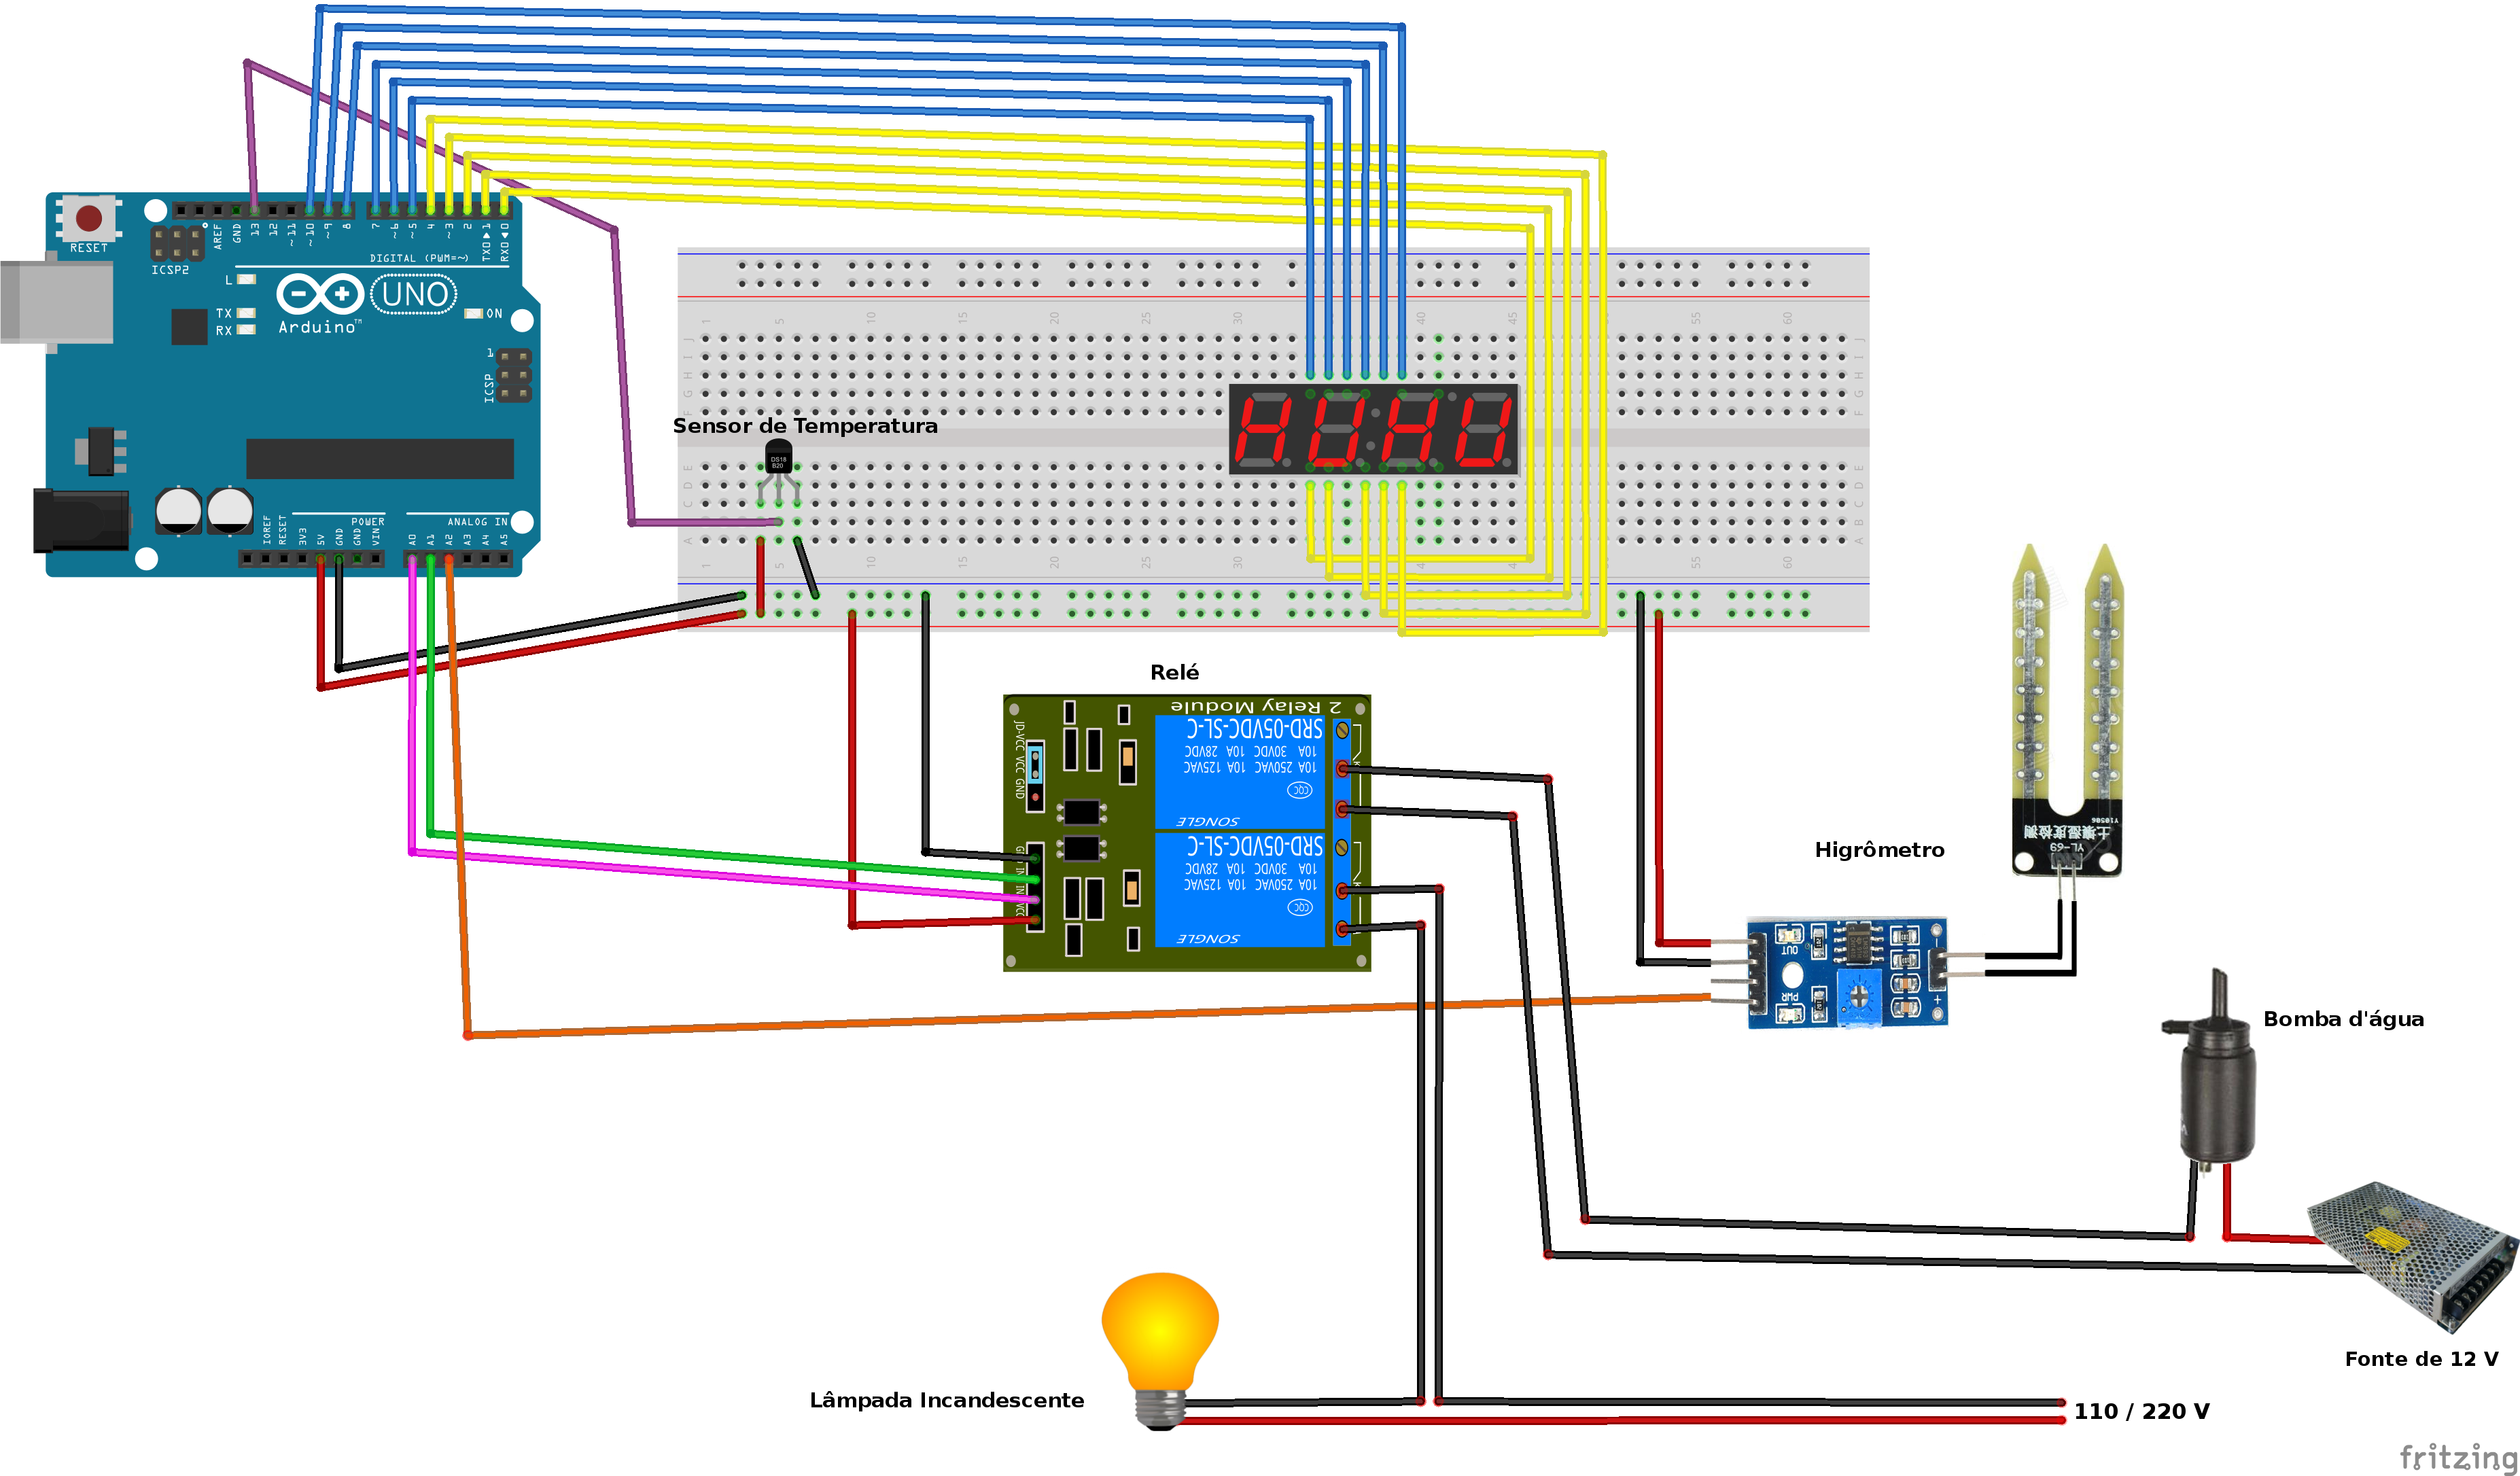
\includegraphics[width=1.15\textwidth]{EsquemaEletronica.png}
		    \caption{Esquema da montagem da eletrônica do projeto.}
		\end{figure}





\section{Procedimentos de Teste e Validação}

    O \textit{Arduino} mostra-se um grande facilitador para as etapas de teste e validação. Antes de se fazer uma montagem completa do projeto, é possível fazer montagens parciais (somente alguns componentes) e testar cada módulo do projeto. Por exemplo, é possível ligar apenas o sensor de temperatura à placa e com um código bastante enxuto é possível utilizar o \textit{Serial Monitor} da \textit{Arduino IDE} para mostrar ao usuário as informações colhidas pelo sensor. A partir daí, é possível criar uma estrutura condicional que execute uma determinada função quando a temperatura estiver a baixo de um determinado limite. Com essa estrutura funcionando, não importa a função que será executada, e essa poderá ser implementada posteriormente, como parte de outro módulo de teste.

    Dessa forma, foi possível desenvolver cada módulo separadamente e integrá-los posteriormente no código-fonte. Iniciamos desenvolvendo um módulo para a utilização do \textit{display} LED, que apesar de parecer simples se mostrou um desafio interessante. Não utilizamos bibliotecas prontas e fizemos uso do \textit{PWM} do \textit{Arduino} para alimentar os LEDs. Isso dispensa o uso de resistores e é uma solução bastante elegante. Em seguida, o módulo a ser desenvolvido e testado foi a ativação do relé. Utilizando um botão, definimos o relé para ativar suas portas quando o estado do botão alternasse. Por fim, foram implementados os módulos dos sensores, que são um pouco mais complexos por envolveram uma calibragem adicional.

    O sensor de temperatura necessita para seu correto funcionamento o uso das bibliotecas externas\texttt{ OneWire.h} e \texttt{DallasTemperature.h}. Essas bibliotecas são utilizadas para detectar a porta de entrada do sensor no \textit{Arduino} e converter o valor de leitura em um valor legível para o ser humano. Por padrão, o valor de temperatura devolvido pelas bibliotecas é na unidade de grau Celsius, o que é a unidade comumente usada no Brasil e a interpretação será facilitada para o usuário. Já o sensor de umidade, mede a tensão encontrada entre as duas hastes da sonda colocada no solo e retorna um valor entre 0 e 1023. Para interpretar esse valor, foi necessário fazer um calibragem empírica; analisando a resposta obtida ao se colocar o sensor em um solo gradativamente umedecido, foi possível verificar como se dava a variação da leitura em função da umidade. Dessa forma, a partir de observações conseguimos definir diferentes faixas de valores que significam solo seco, solo levemente umedecido, solo com umidade moderada e solo úmido. Sendo assim é fácil com poucas alterações no programa definir o quão úmido o programa de controle tentará manter o solo, o que é bastante útil uma vez que diferentes tipos de plantas níveis de água diferentes.

    Uma vez que cada módulo funciona quando isolado do projeto, a etapa final vem ser a de encaixar todos os módulos do sistema e desenvolver um código final que junta todas as partes e as faz funcionar em conjunto. Dado que cada módulo já havia sido implementado e testado, essa etapa não foi um grande desafio. Bastou amarrar a leitura dos sensores com a ativação do relé e a mostragem do \textit{display}.



\section{Análise de riscos}
Os principais riscos do projeto dizem respeito à montagem do mesmo. É necessário ter cautela na hora de manusear ferramentas cortantes durante a preparação dos cabos e do circuito hidráulico, pois é fácil adquirir ferimentos indesejáveis. Cautela é ainda essencial na hora de fazer as emendas eletrônicas (se necessárias) para que não existam cabos descascados salientes, que podem não somente curto-circuitar o sistema como ainda causar choques elétricos no indivíduo. Além disso, muito cuidado é essencial na hora de se trabalhar com a rede elétrica 110/220 V. Essa tensão é suficiente para causar danos físicos severos e um acidente pode até mesmo ser letal. \cite{halliday2008eletro} O risco de curtos-circuitos acidentais acontecerem é iminente em projetos eletrônicos e um curto não planejado pode trazer prejuízos financeiros caso a rede elétrica não ofereça proteção.

    Se forem tomadas medidas de precaução e a montagem for feita adequadamente, o risco durante a execução do projeto é mínimo e consiste em possível pressão excessiva d’água sobre as plantas ou uma proximidade excessiva da lâmpada com o jardim, que pode gerar calor em excesso e prejudicar as plantas.

    Por tratarem-se de componentes eletrônicos de baixo custo, têm-se o risco de falhas no hardware à longo prazo; a umidade, e a integração direto da bomba de água próximo aos eletrônicos; tal como os fatores externos como calor e chuva, podem oxidar ou trazer mal funcionamento ao projeto.



\section{Cronograma do Projeto}
Antes ainda da equipe ter definido qual seria o projeto a ser desenvolvido, as duas primeiras semanas de desenvolvimento foram dedicadas à se familiarizar com o \textit{Arduino} e sua linguagem, executando atividades propostas pelo kit de iniciantes fornecido em sala, bem como a livre exploração utilizando apenas a criatividade para testar as capacidades da plataforma. Uma vez estabelecido o projeto, pode-se dizer que a primeira semana foi dedicada apenas ao planejamento do projeto (especialmente de sua parte física) e a partir de então, a cada uma ou duas semanas nós focávamos em desenvolver um dos módulos do projeto e em todas as semanas também dedicamos esforços para desenvolver a estrutura do projeto (circuito hidráulico, confecção de cabos e emendas, etc). A partir de então, progressivamente, semana a semana fomos desenvolvendo, em ordem, o módulo do \textit{display} LED para mostrar a temperatura, a leitura e aferição do sensor de temperatura e leitura e calibragem do higrômetro (sensor de umidade do solo).

\newpage
\section{Conclusões}
O desenvolvimento do projeto foi bastante didático para os membros da equipe. Como o trabalho envolveu bastante trabalho de cunho prático, não somente as capacidades intelectuais dos alunos foram exercitadas, mas também as habilidades manuais. A liberdade com que o projeto pode ser desenvolvido permitiu que a equipe tivesse a oportunidade de explorar o aprendizado de novas tecnologias de popularidade emergente como a plataforma \textit{git}, com a qual poucos tinha tido contato posteriormente, que é um controle de versão que está se tornando cada vez mais popular entre a comunidade de desenvolvedores e se tornou uma ferramenta bastante útil para manter a organização do projeto.

Muitos alunos começam o curso de engenharia com pouco conhecimento da área de atuação na qual almejam se graduar, então ter disciplinas introdutórias é uma estratégia de ensino bastante válida para imergir o estudante na área técnica. Nesse quesito, o projeto teve um resultado bastante positivo. Foi notável a evolução da perícia com a qual a equipe lidava com o projeto. De iniciantes completos na área de eletrônica foi possível desenvolver bastante habilidade na programação e desenvolvimento de projetos utilizando \textit{Arduino}.

A confecção do ``Controle e Manutenção de Hortas e Jardins de Baixo Custo com \textit{Arduino}”, ou ainda projeto ``greew” (green + grow) como foi apelidado pela equipe foi, além de um grande aprendizado técnico, uma ótima oportunidade para aperfeiçoar a arte de se trabalhar em equipe, explorando diferentes técnicas de desenvolvimento simultâneo, dividindo tarefas e responsabilidades e pensando em conjunto como solucionar os desafios que apareciam durante o desenvolvimento deste trabalho.


%\appendix
%\addcontentsline{toc}{chapter}{REFER\^ENCIAS}

%\bibliographystyle{unsrt}
\renewcommand\refname{}
\bibliographystyle{abnt}

\newpage
\section{Referências Bibliográficas}
\renewcommand\refname{}
\bibliography{referencias}
%\bibliography{periodicos_extenso,abntdoc}
%\bibliography{macros,abntdoc}



\end{document}
